\documentclass[a4paper,12pt]{article} % добавить leqno в [] для нумерации слева
\usepackage[a4paper,top=1.3cm,bottom=2cm,left=1.5cm,right=1.5cm,marginparwidth=0.75cm]{geometry}
%%% Работа с русским языком
\usepackage{cmap}					% поиск в PDF
\usepackage{mathtext} 				% русские буквы в фомулах
\usepackage[T2A]{fontenc}			% кодировка
\usepackage[utf8]{inputenc}			% кодировка исходного текста
\usepackage[english,russian]{babel}	% локализация и переносы
\usepackage{multirow}

\usepackage{graphicx}

\usepackage{wrapfig}
\usepackage{tabularx}

\usepackage{hyperref}
\usepackage[rgb]{xcolor}
\hypersetup{
colorlinks=true,urlcolor=blue
}

%%% Дополнительная работа с математикой
\usepackage{amsmath,amsfonts,amssymb,amsthm,mathtools} % AMS
\usepackage{icomma} % "Умная" запятая: $0,2$ --- число, $0, 2$ --- перечисление

%% Номера формул
\mathtoolsset{showonlyrefs=true} % Показывать номера только у тех формул, на которые есть \eqref{} в тексте.

%% Шрифты
\usepackage{euscript}	 % Шрифт Евклид
\usepackage{mathrsfs} % Красивый матшрифт

%% Свои команды
\DeclareMathOperator{\sgn}{\mathop{sgn}}

%% Перенос знаков в формулах (по Львовскому)
\newcommand*{\hm}[1]{#1\nobreak\discretionary{}
{\hbox{$\mathsurround=0pt #1$}}{}}

%% Графики
\usepackage{tikz}
\usepackage{pgfplots}
\pgfplotsset{compat=1.9}

\usepackage{subcaption}

\date{\today}

\begin{document}

\begin{titlepage}
	\begin{center}
		{\large МОСКОВСКИЙ ФИЗИКО-ТЕХНИЧЕСКИЙ ИНСТИТУТ (НАЦИОНАЛЬНЫЙ ИССЛЕДОВАТЕЛЬСКИЙ УНИВЕРСИТЕТ)}
	\end{center}
	\begin{center}
		{\large Физтех-школа прикладной математики и информатики}
	\end{center}
	
	
	\vspace{4.5cm}
	{\huge
		\begin{center}
			{\bf Отчёт о выполнении лабораторной работы 3.1.1}\\
			
		\end{center}
	}
	\vspace{1cm}
	\begin{center}
		{\large Соболевский Федор Александрович \\
			\vspace{0.2cm}
			Б05-111}
	\end{center}
	\vspace{8cm}
	\begin{center}
		Октябрь 2022
	\end{center}
\end{titlepage}

\section{Аннотация}

В данной работе был исследован магнитомер -- прибор для измерения величины и направления магнитного поля. С помощью магнитометра была измерена горизонтальная составляющая магнитного поля Земли. По результатам измерений величины электрического тока в установке двумя независимыми способами с использованием полученной величины магнитного поля Земли установлено количественное соотношение между единицами электрического тока в системах СИ и СГС.

\section{Теоретические сведения}

\subsection{Общие сведения о магнитометре}

Магнитометр -- прибор для магнитных измерений, например: компас, теодолит, веберметр и пр. С помощью магнитометров измеряют намагниченность ферромагнетиков, напряжённость магнитных полей, исследуют магнитные аномалии. Разработаны магнитометры различных конструкций: магнитостатические, электромагнитные, магнитодинамические, индукционные, резонансные. Эталонные магнитометры позволяют измерять горизонтальную и вертикальную составляющие напряжённости магнитного поля Земли с точностью $10^{-6}$ Э.

В данной работе помощью электромагнитного магнитометра измеряется горизонтальная составляющая земного магнитного поля и абсолютным образом определяется сила тока по его магнитному действию.

\subsection{Экспериментальная установка}

Магнитометр (рис. \ref{fig:setup}) состоит из нескольких последовательно соединённых круговых витков К, расположенных вертикально. В центре кольца К радиусом $R$ на тонкой неупругой вертикальной нити подвешена короткая магнитная стрелка С. Жёстко связанная со стрелкой крыльчатка погружена в масло и служит для демпфирования колебаний.

\begin{figure}[h!]
\begin{center}
    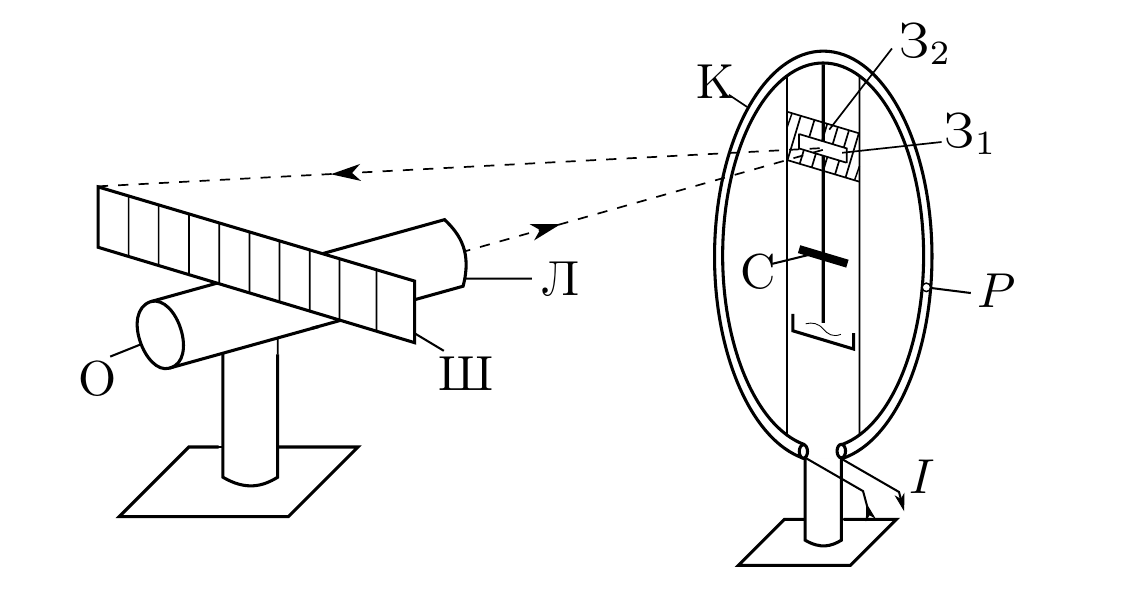
\includegraphics[width=0.7\textwidth]{setup.png}
\end{center}
\caption{Схема устройства магнитометра}
\label{fig:setup}
\end{figure}

\begin{figure}[h!]
\begin{center}
    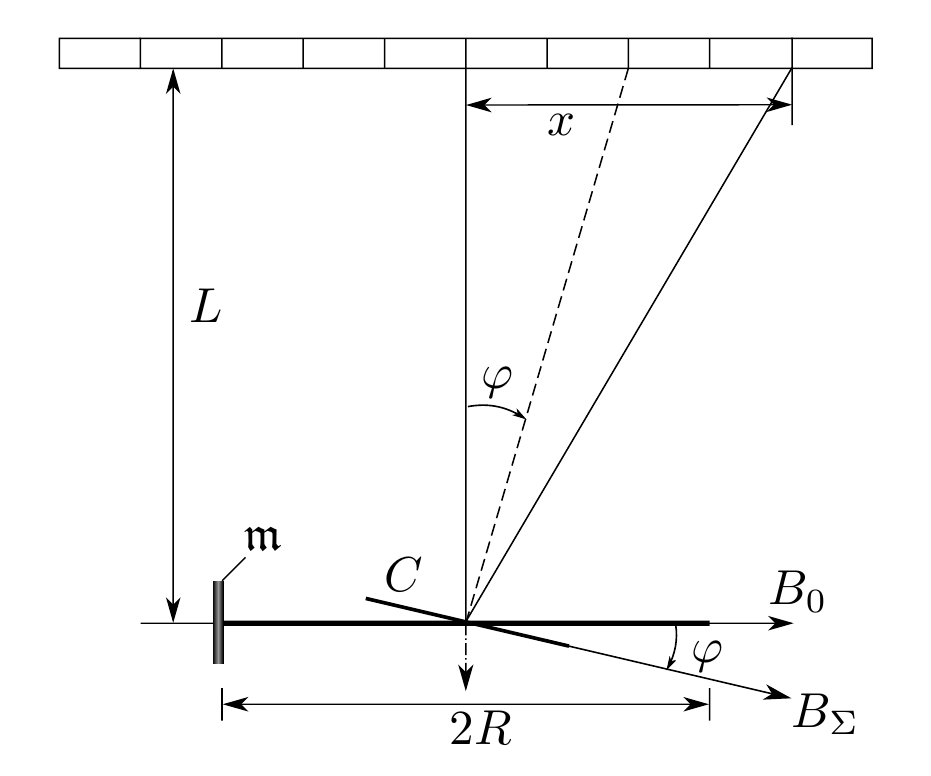
\includegraphics[width=0.6\textwidth]{measurement.png}
\end{center}
\caption{Схема измерения угла отклонения магнитной стрелки}
\label{fig:measurement}
\end{figure}

В отсутствие других магнитных полей стрелка располагается по направлению горизонтальной составляющей земного магнитного поля $B_0$, т. е. лежит в плоскости магнитного меридиана.

Прибор настраивают с помощью световых зайчиков, отражённых от двух зеркал: З$_1$, прикреплённого к стрелке (подвижный зайчик), и З$_2$, расположенного в плоскости кольца К и жёстко связанного с ним (неподвижный зайчик). Оба зеркала освещаются одним и тем же осветителем О. Вращением кольца вокруг вертикальной оси можно совместить оба зайчика. При этом плоскость витков совпадает с плоскостью магнитного меридиана.

При появлении дополнительного горизонтального магнитного поля $B_\perp$ стрелка C установится по равнодействующей обоих полей $B_\Sigma$ (см. рис. \ref{fig:measurement}). В нашей установке дополнительное поле может быть создано либо малым ферромагнитным стержнем, расположенным на кольце на его горизонтальном диаметре ($B_1$), либо током, проходящим по кольцу ($B_2$). В обоих случаях дополнительное поле можно считать однородным, так как размеры стрелки много меньше радиуса кольца. Поле намагниченного стержня вдали от него может быть приближённо вычислено как поле точечного диполя:

\begin{equation}
    \mathbf{B(r)} = \frac{\mu_0}{4\pi}\left(3\frac{(\mathbf{\mathfrak{m} \cdot r})\mathbf{r}}{r^5} - \frac{\mathbf{\mathfrak{m}}}{r^3}\right),
\label{dipoleField}
\end{equation}
где $\mathbf{\mathfrak{m}}$ -- магнитный момент стержня, $\mathbf{r}$ -- радиус-вектор, проведённый из центра диполя в точку наблюдения. На оси, перпендикулярной стержню, имеем

\begin{equation}
    B_1 = \frac{\mu_0}{4\pi}\frac{\mathfrak{m}}{R^3},
\label{perpField}
\end{equation}
где $R$ -- радиус кольца. Магнитное поле в центре кольца с током $I$ по закону Био и Савара равно

\begin{equation}
    B_2 = \frac{\mu_0I}{2R}N.
\label{BiotSavart}
\end{equation}

Здесь $N$ -- число витков в кольце, $I$ -- сила тока в единицах СИ (амперах).

Измерив угол отклонения стрелки $\varphi$, можно связать поля $B_0$ и $B_\perp$ ($B_1$ или $B_2$):

\begin{equation}
    B_\perp = B_0 \cdot \tg\varphi.
\label{angle}
\end{equation}

\subsection{Определение горизонтальной составляющей магнитного поля Земли}

Для определения горизонтальной составляющей земного магнитного
поля $B_0$ тонкий короткий намагниченный стержень устанавливается в
отверстие Р на горизонтальном диаметре кольца (см. рис. \ref{fig:setup}). Измерив тангенс угла отклонения стрелки

\begin{equation}
    \tg\varphi_1 = \frac{x_1}{2L},
\label{angleTan}
\end{equation}

можно с помощью уравнений \eqref{perpField}, \eqref{angle} и \eqref{angleTan} рассчитать поле $B_0$, если исключить величину $\mathfrak{m}$ -- магнитный момент стержня. Для исключения магнитного момента предлагается измерить период крутильных колебаний стержня в поле Земли. Подвешенный горизонтально за середину на тонкой длинной нити стержень в положении равновесия установится по полю Земли (упругость нити пренебрежимо мала). Если ось стержня отклонить в горизонтальной плоскости от
направления $B_0$ на малый угол $\alpha$, то под действием возвращающего механического момента

\begin{equation}
    M_\text{мех} = |\mathbf{\mathfrak{m} \times B}| = \mathfrak{m} B_0 \sin{\alpha} \approx \mathfrak{m} B_0 \alpha
\label{mechMoment}
\end{equation}
стержень с моментом инерции $J$ в соответствии с уравнением гармонических крутильных колебаний

\begin{equation}
    J\ddot{\alpha} + \mathfrak{m} B_0 \alpha = 0
\label{spinOscillation}
\end{equation}
будет совершать крутильные колебания с периодом

\begin{equation}
    T = 2\pi\sqrt{\frac{J}{\mathfrak{m}B_0}}.
\label{period}
\end{equation}

Момент инерции цилиндрического стержня относительно оси вращения

\begin{equation}
    J = m\left(\frac{l^2}{12} + \frac{r^2}{4}\right) = \frac{ml^2}{12}\left[1 + 3\left(\frac{r}{l}\right)^2\right],
\label{inertiaMoment}
\end{equation}
где $m$ -- масса стержня, $l$ -- длина, а $r$ -- его радиус. Таким образом, рассчитав момент инерции $J$ и измерив тангенс угла отклонения стрелки $\varphi_1$ и период малых крутильных колебаний стержня $T$, можно с помощью формул \eqref{perpField}, \eqref{angle}, \eqref{angleTan} и \eqref{period} определить горизонтальную составляющую магнитного поля Земли:

\begin{equation}\label{earthfield}
    B_0 = \frac{2\pi}{TR}\sqrt{\frac{\mu_0 J L}{2\pi Rx_1}} \quad [\text{ед. СИ}].
\end{equation}

\subsection{Определение электродинамической постоянной}

Ток в цепи кольца можно измерить двумя независимыми способами:
по магнитному действию тока на стрелку магнитометра и по заряду,
протекающему через цепь в единицу времени. Первый способ измерения
соответствует тому, как эталон тока определён в системе СИ, а второй -- в гауссовой системе (СГС). По отношению результатов этих измерений можно определить электродинамическую постоянную $c$.

Пропуская некоторый ток через витки магнитометра, измерим тангенс угла отклонения стрелки ($\tg\varphi_2 = x_2/2L$,) и по формулам \eqref{BiotSavart} и \eqref{angle} рассчитаем силу тока:

\begin{equation}
    I = \frac{2B_0 R}{\mu_0 N} \tg\varphi_2 \quad [\text{ед. СИ}].
\label{amperage}
\end{equation}

Величина $A = 2B_0 R/(\mu_0 N)$ является постоянной прибора в данном месте земной поверхности (точнее, в данном месте комнаты -- с учётом многочисленных сторонних источников магнитного поля).

Тот же ток можно измерить абсолютным образом по прошедшему
в единицу времени заряду, что соответствует определению эталона тока в гауссовой системе (СГС). Если разрядить конденсатор известной
ёмкости $C$, заряженный до напряжения $U$, через витки, то через них
протечёт заряд $q = CU$ (рис. \ref{fig:circuit}). Если $\nu$  раз в секунду последовательно заряжать конденсатор от источника и разряжать через витки, то через них за секунду протечёт заряд $CU\nu$. Средний ток, прошедший через витки, равен при этом

\begin{equation}
    I = CU\nu \quad [\text{абс. ед.}].
\label{avCurrent}
\end{equation}

\begin{figure}[h!]
\begin{center}
    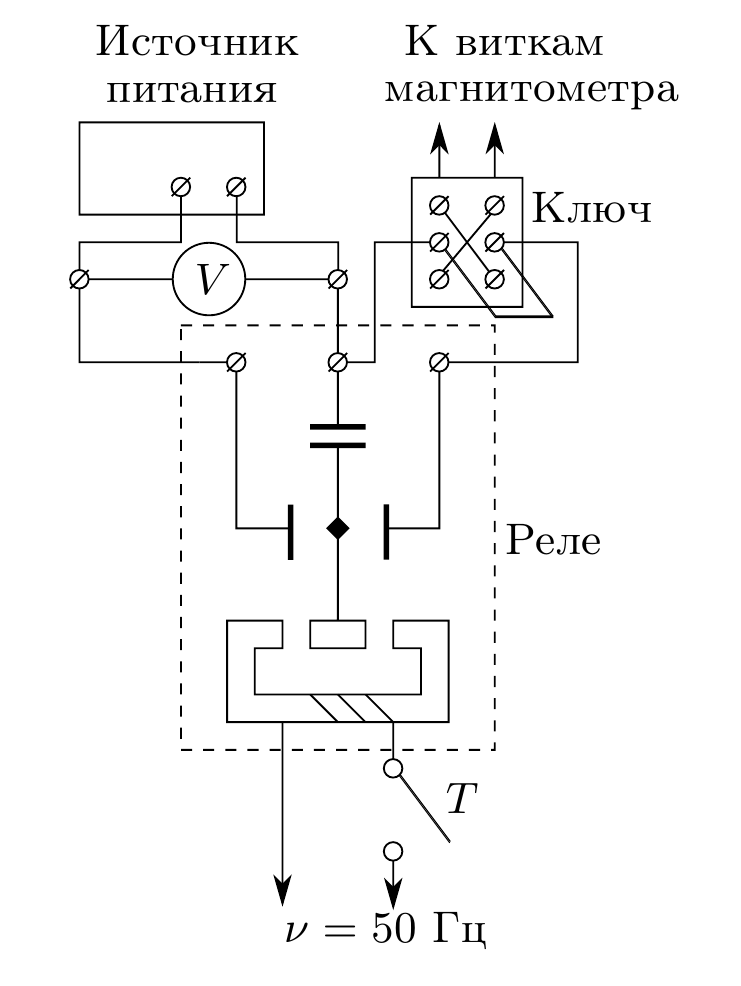
\includegraphics[width=0.4\textwidth]{circuit.png}
\end{center}
\caption{Схема питания катушки магнитометра}
\label{fig:circuit}
\end{figure}

Для вычисления абсолютного значения тока по \eqref{avCurrent} необходимо измерить напряжение $U$ на конденсаторе известной ёмкости $C$. Напряжение необходимо выразить в единицах СГС (измерительные приборы, как правило, проградуированы в единицах СИ: $1 \text{В} \approx \frac{1}{300}$ ед. СГС). Ёмкость конденсатора $C$ [см] должна быть выражена в сантиметрах ($1 \text{Ф} \approx 9 \cdot 10^{11}$ см).

По отношению численных значений одного и того же тока, выраженных в единицах СИ и СГС (гауссовой) по формулам \eqref{amperage} и \eqref{avCurrent} соответственно, можно определить значение электродинамической постоянной:

\begin{equation}
    c = \frac{1}{10}\frac{I_\text{[СГС]}}{I_\text{[СИ]}}.
\label{electroConst}
\end{equation}

\section{Оборудование и инструментальные погрешности}

\textbf{В работе использовались:} магнитометр, осветитель со шкалой, источник питания, вольтметр, электромагнитный переключатель, конденсатор, намагниченный стержень, прибор для определения периода крутильных колебаний, секундомер, рулетка, штангенциркуль.

\textbf{Инструментальные погрешности:}

\begin{itemize}
    \item Измерительная шкала: $\Delta_x = 2$ мм;
    \item Рулетка: $\Delta_L = 2$ см;
    \item Секундомер: $\Delta_T = 0,01$ с;
    \item Штангенциркуль: $\Delta_l = 0,1$ мм;
    \item Вольтметр: $\Delta_U = 1$ В.
\end{itemize}

\section{Результаты измерений и обработка экспериментальных данных}

\subsection{Измерение горизонтальной составляющей магнитного поля Земли}

Параметры магнитометра: $L = 1$ см, $R = 20$ см, $N = 44$ витка, $C = 9\cdot10^5$ см $\pm2\%$, $\nu = 50$ Гц. Параметры магнитного стержня: $m = 5,900\pm0,001$ г, $l = 4,00\pm0,01$ см, $r= 0,245\pm0,010$ см.

Результаты измерений смещения подвижного зайчика $x_{1\pm}$ при добавлении магнитного стержня представлены в таб. \ref{tab:res1}. Видно, что все измеренные значения совпадают в пределах инструментальной погрешности, поэтому полную погрешность измерения можно принять равной инструментальной.

\begin{table}[h!]
\begin{center}
\begin{tabular}{|c|c|c|c|c|c|}
\hline
    № измерения & 1 & 2 & 3 & 4 & 5 \\ \hline
    $x_{1+}$, см & 7,0 & 7,0 & 7,0 & 7,0 & 7,0 \\ \hline
    $x_{1-}$, см & -7,0 & -7,0 & -7,0 & -7,0 & -7,0 \\ \hline
\end{tabular}
\end{center}
\caption{Результаты измерения отклонения магнитометра с намагниченным стержнем}
\label{tab:res1}
\end{table}

При измерении периода крутильных колебаний для достижения точности в более чем 1\% проводить измерения нужно хотя бы в течении $\approx 60$ с, т. е. более 1 минуты. Получаем 20 колебаний за $131,2\pm0,1$ с, следовательно, период 1 колебания равен $6,56\pm0,01$ c.

По формуле \eqref{inertiaMoment} вычисляем момент инерции стержня. Полученное значение: $$J = (8,2\pm0,5) \cdot 10^{-7} \text{ кг}\cdot\text{м}^2.$$

По формуле~\eqref{earthfield} вычисляем горизонтальную составляющую магнитного поля Земли. Полученное значение: $$B_0 = 14,8\pm0,6\text{ мкТл}.$$

\subsection{Измерение электродинамической постоянной}

Результаты измерений отклонения зайчика $x_2$ при пропускании тока через цепь представлены в таб. \ref{tab:res2}. Все значения снова совпадают в пределах погрешности измерений.

\begin{table}[h!]
\begin{center}
\begin{tabular}{|c|c|c|c|c|c|}
\hline
    № измерения & 1 & 2 & 3 & 4 & 5 \\ \hline
    $x_{2+}$, см & 9,0 & 9,0 & 9,0 & 9,0 & 9,0 \\ \hline
    $x_{2-}$, см & -9,0 & -9,0 & -9,0 & -9,0 & -9,0 \\ \hline
\end{tabular}
\end{center}
\caption{Результаты измерений отклонения магнитометра при наличии тока в цепи}
\label{tab:res2}
\end{table}

Напряжение на конденсаторе $U = 89,0\text{ B}$. По формулам \eqref{amperage} и \eqref{avCurrent} рассчитано значение тока в цепи. Полученные значения: $$I_\text{СИ} = (4,8\pm0,3)\cdot 10^{-2}\text{ мА}; \quad I_\text{СГС} = (1,34\pm0,03)\cdot10^7\text{ абс. ед.}$$

По формуле \eqref{electroConst} вычислена электродинамическую постоянную:

$$c = 2,77\pm0,14\cdot10^8 \frac{\text{м}}{\text{с}}.$$

\section{Обсуждение результатов и выводы}

\subsection*{Полученные значения}

В данной работе была измерена горизонтальная составляющая магнитного поля Земли, а также была определена электродинамическая постоянная.

Полученное значение горизонтальной составляющей магнитного поля Земли:
$$\boxed{B_0 = 14,8\pm0,6 \text{мкТл}}$$ соответствует табличному значению $15,97 \text{мкТл}$ в пределах удвоенного стандартного отклонения. Основной вклад в погрешность вносит определение смещения зайчика и параметров магнитного стержня. Ошибка измерений может быть связано с наличием сторонних источников магнитного поля в лаборатории: мобильных телефонов, компьютеров и других электроприборов.

Полученное значение электродинамической постоянной: $$\boxed{c = 2,77\pm0,14\cdot10^8 \frac{\text{м}}{\text{с}}}$$ также соответствует табличному значению $2,99\cdot10^8 \frac{\text{м}}{\text{с}}$ в пределах двух стандартных отклонений. Небольшое отклонение может быть вызвано наводкой от токов в цепи или особенностями экспериментальной установки, а также наличием сторонних источников магнитного поля. Основной вклад в погрешность вносит определение горизонтальной составляющей магнитного поля Земли при расчёте тока по определению системы СИ и определение отклонения зайчика.

\subsection*{Выводы}

Опыт показал, что магнитное поле Земли имеет достаточную силу, чтобы производить видимое воздействие на достаточно точные магнитометры и другие приборы, измеряющие косвенно или непосредственно магнитное поле. При минимизациии количества сторонних источников поля можно достаточно точно измерить величину магнитной индукции поля Земли. Эксперимент с предложенной установкой позволил достаточно точно измерить горизонтальную составляющую данной величины, что говорит о применимости данной установки в качестве магнитометра. Экспериментально также удалось с достаточной точностью установить значение электродинамической постоянной, однако погрешность измерений слишком значительна, чтобы использовать полученное значение для точных вычислений в дальнейшем, поэтому предпочтительно использовать табличные значения.

Самый большой вклад в погрешность измерений внесла небольшая точность измерения угла отклонения магнитометра с помощью солнечных зайчиков и градуированной шкалы. Для повышения точности измерений можно использовать другие приборы для измерения углов, например, крутильные весы или стрелку с измерительной шкалой.

\end{document}
